\documentclass{beamer}
\beamertemplatenavigationsymbolsempty
\usetheme{CambridgeUS}
\begin{document}
\title{2018 PbPb run MB Trigger Studies}
\subtitle{Day 1 Tasks}

%Slide 1
\begin{frame}
\frametitle{CaloTower Energy (Offline) and iet (L1Ntuple) Distribution for abs(ieta) $<$ 28 for 2017 XeXe Empty Bunches Data} 


\begin{figure}
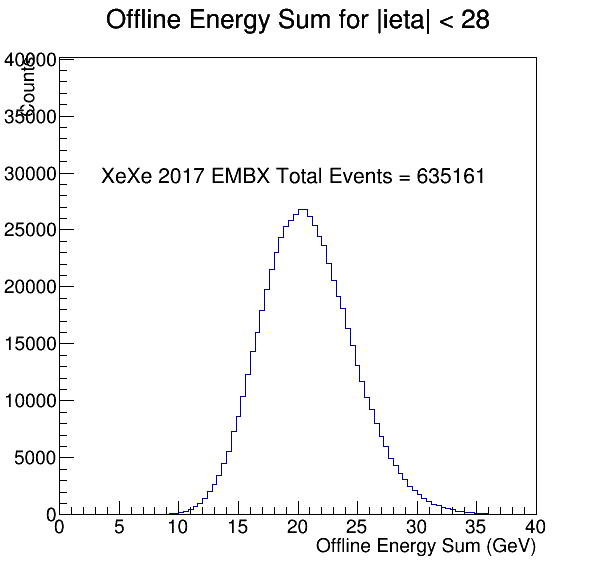
\includegraphics[width=0.38\textwidth]{Plots/XeXe/EnergySumHis28.png}
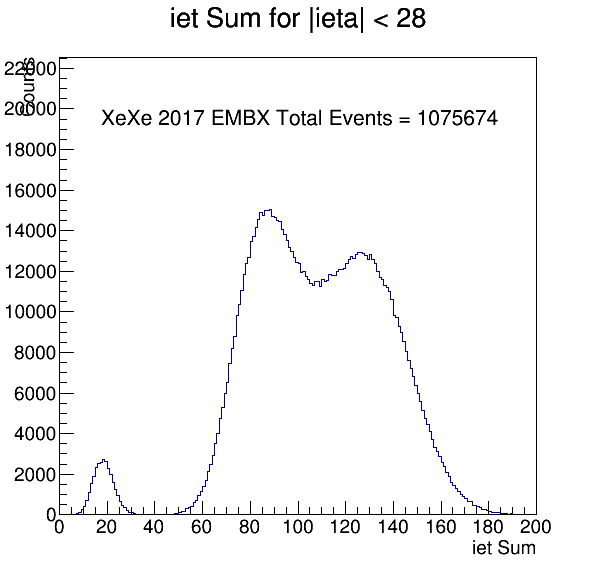
\includegraphics[width=0.38\textwidth]{Plots/XeXe/iETSumHisLT28.png}
\end{figure}

\begin{block}
{Comment: the sum of iet is greater than 100 for $|ieta| < 28$ for XeXe empty bunches data (dataset = /HIEmptyBX/XeXeRun2017-v1/RAW, CMS Release = CMSSW\_10\_1\_5, GT = 101X\_dataRun2\_v8). Therefore, the low EET threshold in MB trigger will not help.}
\end{block}

\end{frame}

%Slide 2
\begin{frame}
\frametitle{CaloTower Energy (Offline) and iet (L1Ntuple) Distribution for abs(ieta) $<$ 25 for 2017 XeXe Empty Bunches Data}

\begin{figure}
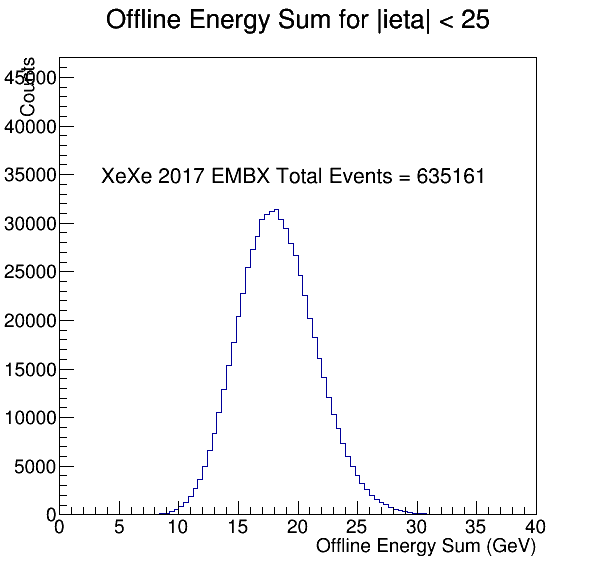
\includegraphics[width=0.38\textwidth]{Plots/XeXe/EnergySumHis25.png}
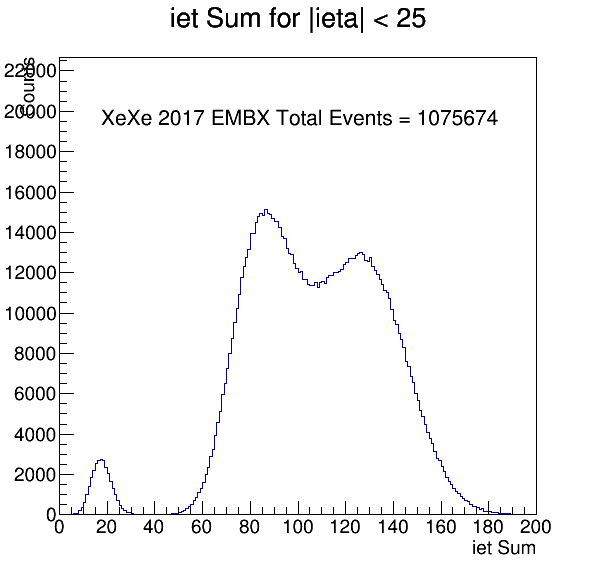
\includegraphics[width=0.38\textwidth]{Plots/XeXe/iETSumHisLT25.png}
\end{figure}


\begin{block}
{Comment: the sum of iet is greater than 100 for $|ieta| < 25$ for XeXe empty bunches data. Therefore, the low EET threshold in MB trigger will not help.}
\end{block}
\end{frame}

%Slide 3
\begin{frame}
\frametitle{iet (L1Ntuple) Sum Distribution for abs(ieta) $<$ 25 and abs(ieta) $<$ 28 for 2018 Low PU pp (July 9 2018) Data} 

\begin{figure}
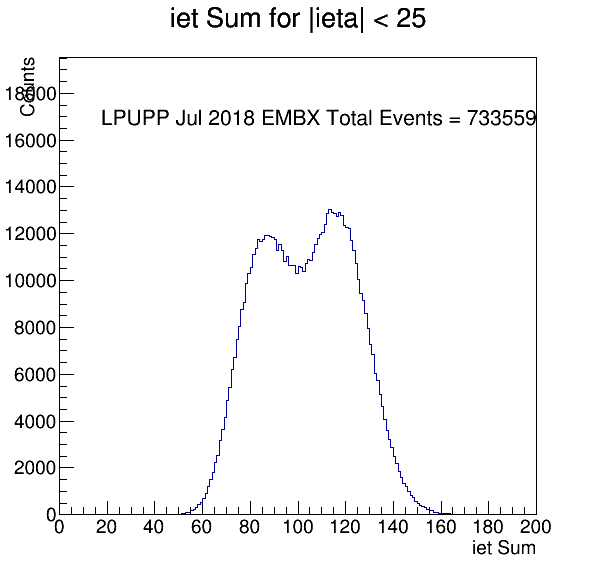
\includegraphics[width=0.38\textwidth]{Plots/pp/iETSumHisLT25.png}
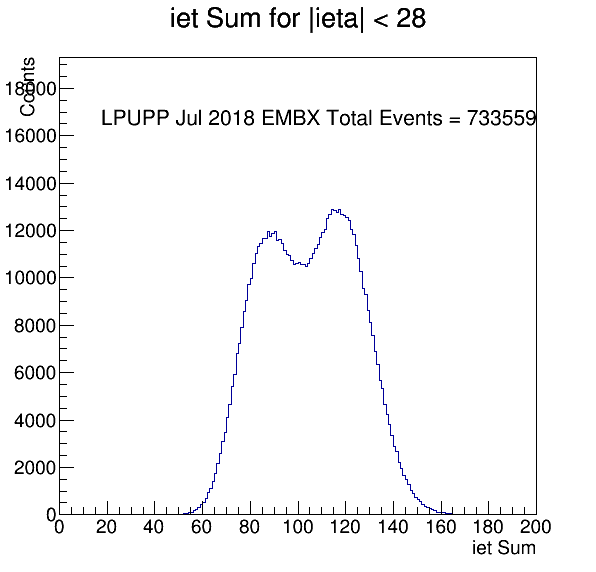
\includegraphics[width=0.38\textwidth]{Plots/pp/iETSumHisLT28.png}
\end{figure}


\begin{block}
{Comment: the sum of iet is greater than 100 for $|ieta| < 25$ and $|ieta| < 28$ for Low PU pp empty bunches data (dataset = /HIEmptyBX/XeXeRun2017-v1/RAW, CMS Release = CMSSW\_10\_1\_5, GT = 101X\_dataRun2\_Prompt\_v9).}
\end{block}
\end{frame}


%Slide 4
\begin{frame}
\frametitle{iet (L1Ntuple) Sum Distribution for abs(ieta) $<$ 25 and abs(ieta) $<$ 28 for 2018 Low PU pp (July 9 2018) Data} 

\begin{figure}
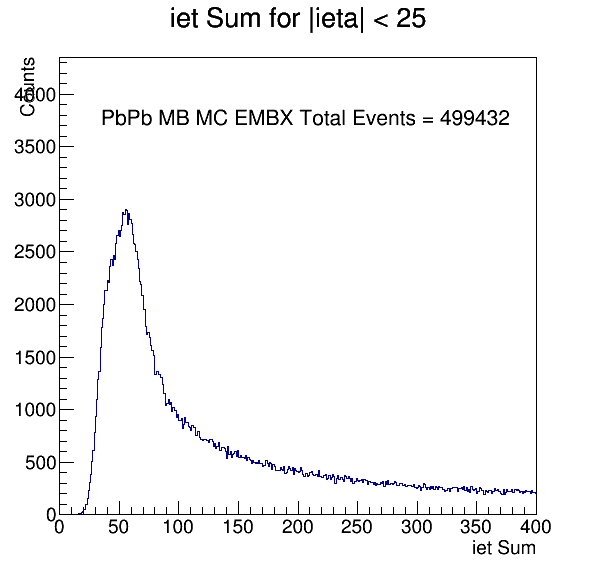
\includegraphics[width=0.38\textwidth]{Plots/PbPb/iETSumHisLT25.png}
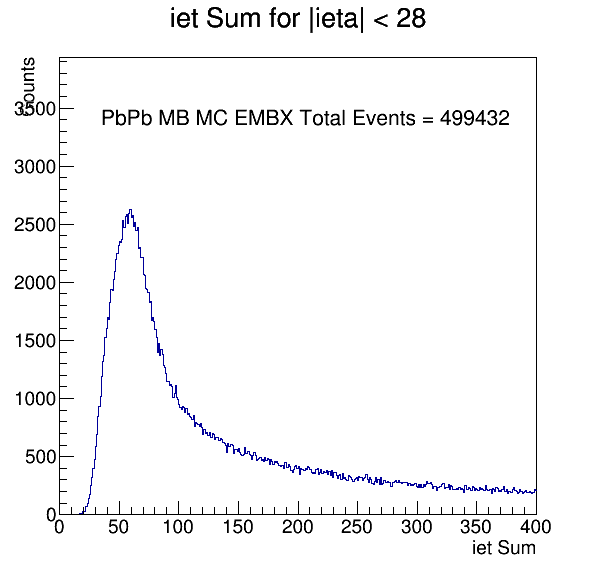
\includegraphics[width=0.38\textwidth]{Plots/PbPb/iETSumHisLT28.png}
\end{figure}


\begin{block}
{Comment: the sum of iet peaks near 60 for $|ieta| < 25$ and $|ieta| < 28$ for PbPb MC MB data (dataset = /HIEmptyBX/XeXeRun2017-v1/RAW, CMS Release = CMSSW\_10\_1\_5, GT = 101X\_dataRun2\_Prompt\_v9). Therefore, the study based on PbPb MC MB data is not reliable for real data.}
\end{block}
\end{frame}


\end{document}